% Options for packages loaded elsewhere
\PassOptionsToPackage{unicode}{hyperref}
\PassOptionsToPackage{hyphens}{url}
\PassOptionsToPackage{dvipsnames,svgnames,x11names}{xcolor}
\documentclass[
  english,
]{scrreprt}
\usepackage{xcolor}
\usepackage{amsmath,amssymb}
\setcounter{secnumdepth}{5}
\usepackage{iftex}
\ifPDFTeX
  \usepackage[T1]{fontenc}
  \usepackage[utf8]{inputenc}
  \usepackage{textcomp} % provide euro and other symbols
\else % if luatex or xetex
  \usepackage{unicode-math} % this also loads fontspec
  \defaultfontfeatures{Scale=MatchLowercase}
  \defaultfontfeatures[\rmfamily]{Ligatures=TeX,Scale=1}
\fi
\usepackage{lmodern}
\ifPDFTeX\else
  % xetex/luatex font selection
  \setmainfont[]{Linux Libertine O}
  \setsansfont[]{Linux Biolinum O}
\fi
% Use upquote if available, for straight quotes in verbatim environments
\IfFileExists{upquote.sty}{\usepackage{upquote}}{}
\IfFileExists{microtype.sty}{% use microtype if available
  \usepackage[]{microtype}
  \UseMicrotypeSet[protrusion]{basicmath} % disable protrusion for tt fonts
}{}
\makeatletter
\@ifundefined{KOMAClassName}{% if non-KOMA class
  \IfFileExists{parskip.sty}{%
    \usepackage{parskip}
  }{% else
    \setlength{\parindent}{0pt}
    \setlength{\parskip}{6pt plus 2pt minus 1pt}}
}{% if KOMA class
  \KOMAoptions{parskip=half}}
\makeatother
\usepackage{longtable,booktabs,array}
\usepackage{calc} % for calculating minipage widths
% Correct order of tables after \paragraph or \subparagraph
\usepackage{etoolbox}
\makeatletter
\patchcmd\longtable{\par}{\if@noskipsec\mbox{}\fi\par}{}{}
\makeatother
% Allow footnotes in longtable head/foot
\IfFileExists{footnotehyper.sty}{\usepackage{footnotehyper}}{\usepackage{footnote}}
\makesavenoteenv{longtable}
\usepackage{graphicx}
\makeatletter
\newsavebox\pandoc@box
\newcommand*\pandocbounded[1]{% scales image to fit in text height/width
  \sbox\pandoc@box{#1}%
  \Gscale@div\@tempa{\textheight}{\dimexpr\ht\pandoc@box+\dp\pandoc@box\relax}%
  \Gscale@div\@tempb{\linewidth}{\wd\pandoc@box}%
  \ifdim\@tempb\p@<\@tempa\p@\let\@tempa\@tempb\fi% select the smaller of both
  \ifdim\@tempa\p@<\p@\scalebox{\@tempa}{\usebox\pandoc@box}%
  \else\usebox{\pandoc@box}%
  \fi%
}
% Set default figure placement to htbp
\def\fps@figure{htbp}
\makeatother
\ifLuaTeX
\usepackage[bidi=basic,shorthands=off,]{babel}
\else
\usepackage[bidi=default,shorthands=off,]{babel}
\fi
\ifPDFTeX
\else
\babelfont{rm}[]{Linux Libertine O}
\fi
\ifLuaTeX
  \usepackage{selnolig} % disable illegal ligatures
\fi
\setlength{\emergencystretch}{3em} % prevent overfull lines
\providecommand{\tightlist}{%
  \setlength{\itemsep}{0pt}\setlength{\parskip}{0pt}}
\usepackage{calc}
\usepackage{hhline}
\usepackage{multirow} 
\usepackage{colortbl}
\usepackage{xcolor}

\lowertitleback{© 2009–2016 Lehrstuhl für Religionswissenschaft, Ruhr-Universität Bochum

\bigskip
unter Mitarbeit von Ann-Kathrin Wolf

\bigskip
5. Auflage\\
Stand: \today

\bigskip
Gesetzt mit Xe\LaTeX
}

\newlength{\iconwidth}
\setlength{\iconwidth}{1cm}

\definecolor{boxheadcol}{gray}{.6}
\definecolor{boxcol}{gray}{.9}

\newenvironment{displaybox}[2]{%
    \begin{center}
        \setlength\arrayrulewidth{0.75pt}%
        \arrayrulecolor{white}%
        \renewcommand{\arraystretch}{1.3}%
        \begin{tabular}{p{\iconwidth}p{\linewidth-4\tabcolsep-\iconwidth}}
            \multirow{2}{*}{#2}&\cellcolor{boxheadcol}\textbf{\sffamily\color{white}#1} \\%
            \hhline{~-}%
            &\cellcolor{boxcol}%
}{%
            \\
        \end{tabular}
        \arrayrulecolor{black}
    \end{center}
}

\newenvironment{Tipp}{%
\begin{displaybox}{Tipp}{
\includegraphics[width=\iconwidth]{images/icon-tipp}}}%
{\end{displaybox}}

\newenvironment{Hinweis}{%
\begin{displaybox}{Hinweis}{
\includegraphics[width=\iconwidth]{images/icon-hinweis}}}%
{\end{displaybox}}

\newenvironment{Technik}{%
\begin{displaybox}{Technik}{
\includegraphics[width=\iconwidth]{images/icon-technik}}}%
{\end{displaybox}}

\newenvironment{Merke}{%
\begin{displaybox}{Merke}{
\includegraphics[width=\iconwidth]{images/icon-merke}}}%
{\end{displaybox}}

\newenvironment{Beispiel}{%
\begin{displaybox}{Beispiel}{
\includegraphics[width=\iconwidth]{images/icon-beispiel}}}%
{\end{displaybox}}

\newenvironment{Tip}{%
\begin{displaybox}{Tip}{
\includegraphics[width=\iconwidth]{images/icon-tipp}}}%
{\end{displaybox}}

\newenvironment{Advice}{%
\begin{displaybox}{Advice}{
\includegraphics[width=\iconwidth]{images/icon-hinweis}}}%
{\end{displaybox}}

\newenvironment{Technology}{%
\begin{displaybox}{Technology}{
\includegraphics[width=\iconwidth]{images/icon-technik}}}%
{\end{displaybox}}

\newenvironment{Remember}{%
\begin{displaybox}{Remember}{
\includegraphics[width=\iconwidth]{images/icon-merke}}}%
{\end{displaybox}}

\newenvironment{Example}{%
\begin{displaybox}{Example}{
\includegraphics[width=\iconwidth]{images/icon-beispiel}}}%
{\end{displaybox}}
\usepackage{bookmark}
\IfFileExists{xurl.sty}{\usepackage{xurl}}{} % add URL line breaks if available
\urlstyle{same}
\hypersetup{
  pdftitle={A Guide to Academic Writing in Religious Studies},
  pdfauthor={Frederik Elwert; Anna Neumaier},
  pdflang={en},
  colorlinks=true,
  linkcolor={Maroon},
  filecolor={Maroon},
  citecolor={Blue},
  urlcolor={Blue},
  pdfcreator={LaTeX via pandoc}}

\title{A Guide to Academic Writing in Religious Studies}
\author{Frederik Elwert \and Anna Neumaier}
\date{}

\begin{document}
\maketitle

{
\hypersetup{linkcolor=}
\setcounter{tocdepth}{1}
\tableofcontents
}
\chapter{Types of Academic Texts}\label{types-of-academic-texts}

Academia takes place predominantly in the medium of language, and texts will play a central role in your studies: knowledge is conveyed in the form of texts, academic sources are read, classified, and acquired. What has been learned is also presented in written form, e.g.~in term papers (\emph{Hausarbeiten}) and exams.

\section{Types of Assignments}\label{sec:assignments}

A large component of course assignments are in written form. In order to be able to meet the requirements of the various kinds of written assignment, one must be familiar with them. Assignments written during the course of study differ not only in length, but also in their purpose, structure and style.

The longest form of assignment - apart from the final thesis - is a term paper (\emph{Hausarbeit}). Term papers in BA studies usually comprise 12-18 pages, whereby usually six pages are credited with 1 CP each. The term paper represents an independent academic achievement, something that is reflected in the requirements.

For a term paper a student should work independently on a chosen topic. This includes the literature consultation and presentation of the state of research, as well as the formulation of a clear structure and answering an independently developed research question. A term paper must also meet certain formal requirements, such as correct citation style and the creation of a bibliography. For more details see section \hyperref[sec:term_papers]{Term Papers}.

A presentation (\emph{Referat}) has a different objective than a term paper. It should not so much deal with a question, which was developed by oneself, but rather give an overview of a certain topic. However, the formal requirements are the same as for a term paper.

It is sometimes possible to arrange to write a term paper as an extension of a presentation, which should then address an independently developed research question. See more details in section \hyperref[sec:presentations]{Lectures and Presentations}.

An essay is a discussion of a given topic. It is less formal and less strict in structure than a term paper. An explicit structure is not usually necessary, and the state of research does not have to be comprehensively presented. If the essay only refers to one or two sources, the citations can also become less important.

An important feature of the essay is the well-argued examination of a topic. While questions of structure are less important, stress is accordingly placed on the quality of argumentation. The essay serves to test argumentative strategies and to present one’s position. An academic position is not to be confused with an opinion: the essay should present a position which the author takes as their own and which is justified soundly in the essay’s arguments. It thus trains its author to develop and organize their own ideas, and at the same time to deal critically with other points of view.

\begin{Tip}

Think about the structure of your arguments before you start writing. For a clear structure and precise language, it can be helpful to create a short outline or mind map which can form the central thread of your writing. This is also useful for term papers or presentations.

\end{Tip}

In university, there are also different types of protocols - experimental or observation protocols in research, but also protocols of seminars, which usually record a session as a mixture of progress and result protocols. This ensures that the results of the meeting are available to all participants, and must therefore be comprehensible to anyone who was not present at the meeting. They are also often a good way of giving feedback to the lecturer, showing which components of the class were absorbed and understood. Meanwhile, writing protocols is a good way of making your personal notes as efficient and precise as possible. A protocol does not have to reflect the course of events in a strict and detailed manner, rather priority is given to summarizing and structuring the key points of the seminar/lecture. This may involve including points made by participants in a class as well as the content of presentations or a lecture. Record should be included of open questions that might be formulated at the end of the session, and of any key sources and/or literature involved. Use of diagrams may often be a helpful tool.

\begin{Tip}

Write the protocol as soon as possible after the session - your notes will be more meaningful when the memory is still fresh! If you have any questions or difficulties in understanding, contact the lecturer or the presenters as soon as possible, preferably directly after the session.

\end{Tip}

Like the protocol, the text summary or excerpt does not constitute an independent academic achievement. The aim of a summary is instead to reproduce the core statements of a text in as concise and precise a form as possible. For more details see the section \hyperref[sec:summaries]{Summaries}.

There are additional forms of written assignment. These can be, for example, reviews, posters or Wikipedia articles. In all cases it is advisable to discuss the performance requirements with the lecturer in order to avoid any misunderstandings.

\begin{Advice}

The following information must be included in the document header of all written assignments in this or a similar form:

Ruhr-Universität Bochum

Center for Religious Studies (CERES)

Course of Studies: MA Religious Studies

\textless Name of the course\textgreater{} \textless Semester\textgreater{}

\textless Name of the lecturer\textgreater{}

\textless name of the author(s)\textgreater{}

\textless Date\textgreater{}

\end{Advice}

\section{Forms of Academic Literature}\label{sec:forms}

In addition to the assignments to be written by students themselves, texts written by scholars play a central role in their studies. Such academic literature can take a variety of forms:

The classic form of the academic text is the monograph, the independent book. Monographs are written by one or more authors on a particular topic. The major academic qualifications such as the doctoral thesis and the habilitation thesis are published in the form of monographs.

An anthology or edited volume is a collection of essays by different authors based around an overall topic. Usually, one refers to individual articles from an anthology, not to the volume as a whole.

Periodicals or journals contain various articles by different authors. The only thing they have in common is often the subject area of the journal itself, but there also exist special issues of journals on a particular theme. Such issues are thus very similar to anthologies.

Manuals differ from anthologies in that the articles they contain are not primarily current research contributions by the authors, rather they present the state of research on a given topic. Also, the articles in manuals are usually shorter.

Dictionaries contain a large number of short articles, usually sorted alphabetically.

Another category is reviews, whether of monographs, anthologies or other works. They contain both a brief description of the content of the reviewed work and a critical analysis thereof with regard to the current state of research.

\chapter{\texorpdfstring{Term Papers (\emph{Hausarbeiten})}{Term Papers (Hausarbeiten)}}\label{sec:term_papers}

\section{Steps of Academic Writing}\label{sec:steps}

The writing of an academic paper is not limited to the writing of the text itself. Both before and after this there are a number of important steps that must be taken into account when planning a paper.

\subsection{Time-Management}\label{time-management}

It is advisable to work out a schedule for the paper before starting the writing process. Especially when it comes to the locating and review of relevant literature, this can often take more time than might be initially assumed. If the required books have been borrowed by someone else or even have to be ordered via interlibrary loan, it can take several weeks until they are available. The further steps also take time. And last but not least, there should be enough time at the end to proofread the work (or have it proofread).

An overall schedule can be helpful for the coordination of different assignments, for example during the semester breaks. It enables more effective use of the limited time available. In addition, a schedule can have motivating effects by showing the points already successfully completed during the course of writing a paper.

\begin{Advice}

Papers are usually written during the semester break. Please bear in mind that during this time office hours are often offered at different times and/or less frequently, and lecturers may also be on holiday. If necessary, it is therefore best to arrange consultation appoint-ments at the end of the teaching period.

\end{Advice}

\subsection{Finding a Topic and Formulating a Question}\label{finding-a-topic-and-formulating-a-question}

The first step in writing an academic paper is to find a topic. In so doing, it is not enough only to identify the issues which the paper will address. It is also necessary to formulate a question that makes it possible to work on the topic with an approach specific to religious studies. Developing a research question is certainly a demanding task. A good question does not usually stop at asking how things can be described (this usually results in a simple reproduction of one’s readings with no critical input), rather an academic question aims at explaining the facts or their consequences. An exception to this can be language-focused research, where the reading and representation of the material is a demanding task in itself.

A second challenge is to narrow down the subject. Topics such as “The History of Hinduism in India” or “The Religiosity of Muslim Youth in Germany” are simply too broad to be dealt with in the context of term papers or even a Bachelor’s thesis. The identification of a topic is also difficult because it requires basic knowledge of the subject in advance. Only then is it possible to determine the more concrete questions into which a topic can be broken down.

Therefore, finding the right topic cannot be done at the desk alone. It requires an initial, rough overview of the available literature and the state of research, as well as conversation with the lecturer. Do not hesitate to tell the lecturer your own ideas, but also be prepared to listen. If you have already acquired some basic knowledge, you can take up the lecturer’s suggestions and work them in sensibly.

\begin{Tip}

Often you can start from a problem that you have encountered in a seminar or even outside the university. For your paper it is essential to make the problem manageable by formulating a clear question. It can be helpful to create a mind map on which you try to set out and structure different aspects of the topic. You only have to concentrate on one of these aspects - the more precise and narrow your question becomes, the easier it will be to work on it.

\end{Tip}

\begin{Example}

The definition of a ‘religious community’ is apparently controversial, as the debate on Scientology shows. The question “What is a religious community?” would be too broad to be answered in a term paper. Moreover, normative approaches - for instance “Why Scientology is not a religious community” - are inappropriate in academic papers. It would be possible to raise a question that picks out one of many aspects, namely the legal debate surrounding this issue: “Which argumentations are used in court decisions about the recognition of religious communities?” The title of the paper could then be:”Judicial argumentations in determining the status of ‘religious community’. An investigation into the example of Scientology.”

\end{Example}

\subsection{Outline and Selection of Literature}\label{outline-and-selection-of-literature}

An initial outline can be established immediately after the research question has been formulated. This allows one to explicate the basic scheme of the work without getting lost in the details of the material. The outline is also the basis for the selection of literature. Only when the approximate direction of the research is known is it possible to then determine which literature is relevant. In addition to literature on the subject, it is often necessary to have an insight into the theoretical literature in order to provide a background for the research question. In a second part of the assignment, depending on the focus of the topic, students can analyse their own selection of sources.

\begin{Example}

The outline of your Scientology term paper might now look like this:

\begin{enumerate}
\def\labelenumi{\arabic{enumi}.}
\item
  Introduction
\item
  (Descriptive part)

  2.1 About Scientology

  2.2 Overview of conflicts and court trials that have taken place
\item
  (Analytical part)

  3.1 Analysis of documents and legal rulings

  3.2 Reference to religious studies literature on Scientology
\item
  Conclusion
\end{enumerate}

\end{Example}

For more details, see the section on \hyperref[sec:outline]{Outline of Chapters}.

\subsection{Literature Consultation and Reading}\label{literature-consultation-and-reading}

Sufficient time should be planned for the literature consultation. Relevant works may already be on loan or even have to be ordered via interlibrary loan. It is therefore advisable to acquire an overview of the required literature at an early stage. (For details of this process, see the section on \hyperref[sec:literature_consultation]{Literature Consultation}.) The range of inquiry is always the current state of research: the texts on a topic are not chosen arbitrarily, but should reflect the particular research area. Of course, it is not possible to reproduce the entire literature on a topic in one paper. However, the selected texts should always be embedded in a context: Which research area do they originate from? To which texts and/or authors do they refer? What other research areas are there that are not considered in the paper? A short overview of the state of research and the existing literature should therefore always be presented at the beginning of your text, for example after the introduction.

The actual work then follows with the reading and evaluation of the selected literature. Again, it is important not to rush into the literature without prior consideration. The reading should also be done with the research question in mind. What kind of argument does the author pursue? Does it agree with your own approaches? If not, can your own approach be justified or should you adapt your theses?

For more details see the sections on \hyperref[sec:literature_consultation]{Literature Consultation} and \hyperref[sec:reading_techniques]{Reading Techniques}.

\subsection{Writing the Paper}\label{writing-the-paper}

Most of the work is done with the writing of the actual text of your assignment. However, if the previous steps have been thoroughly completed, the effort involved in the actual writing of the paper is reduced considerably. Ideally, one should have a clear question and a clear outline, know the literature and just need to get started. One should not only have the layout of the chapters in mind, but also the rough structure of the argument. In this way any weaknesses in structure will become apparent early on, and not only after the assignment has been written.

\begin{Tip}

Write out a basic plan of your term paper, including the structure of your arguments. This will make it much easier to write. You can also include the literature to be used and/or any especially appropriate quotations.

\end{Tip}

After writing the text, you have to spend some time on post-processing. The text should at least be proofread for consistency of content and for any formal errors (spelling, grammar). It is helpful to have someone else proofread the text, because after having worked on it for some time, one becomes blind to many flaws and errors.

\begin{Technology}

Appearance, i.e.~a neat layout, is also part of an academic paper. Here, too, you can reduce subsequent work to a minimum if you work properly from the start. This includes creating an automatically generated table of contents and bibliography. For more details see the sections on \hyperref[sec:word_processing]{Word Processing} and \hyperref[sec:literature_administration]{Literature Administration}.

\end{Technology}

\section{Structure of a Paper}\label{sec:structure}

A term paper must meet certain formal criteria. In addition, there are a number of guidelines regarding the structure, which should be followed.

\subsection{Cover Sheet}\label{cover-sheet}

At the front of each term paper there must be a cover sheet containing several important pieces of information. The cover sheet should present this information as clearly as possible. It must contain:

\begin{itemize}
\item
  Name of the university, faculty and subject of study
\item
  purpose of the paper (e.g.~“Term Paper as Module Examination …” or “essay as examination for the module part …”)
\item
  title, course number and semester of the seminar/module as well as the names of the lecturers
\item
  title of the paper
\item
  name, matriculation number, combination of subjects, number of semesters, address, telephone number, and email address
\item
  date on which the work is submitted
\end{itemize}

The figure shows an example of a cover sheet.

\begin{figure}
\centering
\pandocbounded{
\includegraphics[keepaspectratio]{images/Muster_Cover_Sheet.pdf}}
\caption{Example of a cover sheet}
\end{figure}

\subsection{Table of Contents}\label{table-of-contents}

The table of contents contains the chapters and subchapters of the paper with page numbers. The table of contents itself should not be listed. Many word processing programs support the automatic creation of a table of contents. For more information, see the section on \hyperref[sec:word_processing]{Word Processing}.

\subsection{Outline of Chapters}\label{sec:outline}

Each paper consists of an introduction, a main body and a conclusion. In the introduction the topic of the paper, the question and the structure of the paper are presented. Thus, the reader can already anticipate a certain structure and does not have to deduce it from the text. The main body then contains a sketch of the literature or the state of research and, as the most important part, the student’s actual work on the topic. Finally, the text is briefly summarized once again and the main findings are noted. The conclusion contains no new information or arguments.

However, this structure generally does not fully correspond to the outline of chapters. While the introduction is often called “Introduction”, and the conclusion is likely to be found under the heading “Conclusion” or similar, the main part usually consists of several chapters. The chapters of the main part should reflect the structure of the paper well and be named accordingly, so that the outline of the chapters already gives a good impression of the main topics. Sub-chapters can be divided into smaller sections, but the outline should not be too detailed. In practice, it is often best to divide the main section into three parts, but this is only a rule of thumb: the chapters and sub-chapters should not be unconnected but should be linked together in a meaningful way.

Decimal classification is suitable for the outline of chapters: chapters numbered with 1, 2, and so on, sub-chapters with 1.1, 1.2, etc. An outline level must never contain only a single chapter: If there is a chapter 2.1, then there must also be 2.2.

The individual parts should roughly follow the following structure:

\begin{itemize}
\item
  Introduction to the topic, for example by linking it to historical or general debates
\item
  Presentation of the subsequent topic of the paper and, if applicable, reasons for the choice of topic
\item
  Limitation of the subject area: which aspect of the problem is relevant and can be treated meaningfully in the context of the paper, and which aspects must be left out?
\item
  Formulation of a research question or project, explication and justification (e.g., research gap, relevance for research in religious studies, etc.)
\item
  Description of the procedure and structure of the paper
\item
  Short overview of the literature used in the context of the state of research and possibly the sources
\end{itemize}

\begin{Tip}

Imagine the introduction of a paper as being like a funnel: you start broadly, with a reference to a generally relevant issue, and then narrow it down to your chosen problem. This approach has its counterpart in the conclusion - here the findings of the paper are again opened up into a more general debate.

\end{Tip}

\begin{itemize}
\item
  Presentation and execution of the preceding arguments, answering the question raised in the introduction.
\item
  Reproduce the researched and selected literature and discuss divergent approaches and arguments; do not retell the content, but select specific focal points based on the question posed.
\item
  Back up your statements with meaningful examples and quotations; pay attention to the corresponding citations in the footnotes.
\end{itemize}

\begin{itemize}
\item
  Summarize the presentation and argumentation of the text briefly, and gather everything together in the formulation of a result that you have arrived at.
\item
  If necessary (especially in empirical work), critically reflect on your own approach: Was the method useful? Has anything remained open or unclear?
\item
  Concluding statement on the topic: significance of your own results - both for your specific question and for the general topic.
\item
  Outlook regarding further questions which your work could not answer or which your results have raised for further research.
\end{itemize}

\begin{Advice}

The conclusion does not provide any new information that has not already been dealt with in the main part (citations are therefore generally no longer necessary here).

\end{Advice}

\begin{Tip}

If you have written a neatly structured introduction, you can now “backtrack” the other way round - from the specifics of your work to the generalities of a larger debate. In any case, it is important that you refer to the introduction - in this way you make your work coherent and make it clear to the reader that you have written a well-structured and precise academic paper.

\end{Tip}

\subsection{Bibliography and Appendices}\label{bibliography-and-appendices}

At the end of the paper there should be a complete list of all literature used. The bibliography should not be filled up with literature that is not cited in the text. If a publication is important in terms of content, it should be cited, otherwise it does not have to be included in the bibliography. For the formatting of the bibliography see the section \hyperref[sec:citing]{Citing Literature}.

Papers that are rich in material can also contain one or more appendices, in which e.g.~illustrations, source texts or similar can be placed. The appendices do not count for determining the length of the paper.

\subsection{Formatting}\label{formatting}

A term paper in standard format usually contains about 12-18 pages or 5,000-7,000 words. However, the obligatory details are determined by the lecturers. The following guidelines apply to all papers:

\begin{itemize}
\item
  font size 12pt
\item
  line spacing 1.25 to 1.5
\item
  Right margin 4cm - for notes and corrections; left margin 2cm, top/bottom 2-3cm
\item
  Detached headings with section numbers
\item
  Footnotes at the bottom of the page (no endnotes)
\item
  Page numbering from the second page onwards (the title page counts as page 1, but should not have a page number on it)
\item
  Text in justification with (automatic) hyphenation
\end{itemize}

\begin{Technology}

For formatting a term paper with common word processing programs see section \hyperref[sec:word_processing]{Word Processing}.

\end{Technology}

\subsection{Language}\label{language}

Good linguistic expression is also part of a successful paper. Contrary to common assumptions, language is not more academic if it uses many foreign words and complex sentences. The use of technical terms should make a text more precise and - for experts in the field, including the markers - more comprehensible, not less comprehensible. Above all, make sure that you yourself understand what you are writing.

Be precise and specify to whom you are referring, e.g.~by saying: “The author considers that …”. Likewise, you should avoid the first person when you present facts or others’ theories; the first person is reserved for your own arguments or opinions.

Write in a clear way such that no more words could be deleted from your sentences. Filler words like “actually”, “quite”, “to a certain extent” or ” eventually” take away persuasive power from your arguments because they weaken their significance. It is better to write your work in such a way that all statements are fully intended as they are written there. If there are limitations to be considered, they should be made explicit and explained.

The argumentation of the work should also be reflected in the language: Causal links are an important means of connecting your arguments conclusively. However, a common mistake is to make causal links in places where they do not belong. Check very carefully whether sentences or parts of sentences that start with “therefore”, “nevertheless”, “in view of” or other phrases that refer to what has preceded them really do relate appropriately and clearly to what precedes.

Particularly with longer sentences, it is easy to come across incorrect grammatical constructions. Make sure that all formulations, connectors and relations are correct. It is also important to have correct and consistent orthography and punctuation.

For improved readability, the text should be structured with paragraphs. However, a new paragraph should be deliberately added when a new aspect is addressed. Putting each sentence in a separate paragraph is just as unhelpful as a text without paragraphs.

\section{Marking Criteria for Term Papers}\label{sec:marking}

CERES lecturers follow a catalogue of criteria when marking written work. This will be made transparent in order to enable students to self-evaluate their written performance and to make the grading of their work comprehensible.

Generally, the work of the early phases of study should already try to follow this standard. However, these criteria are only applied in their entirety from the BA thesis onwards. The criteria are as follows:

– Quality of research – Expertise – Level of reflection – Consistency of argumentation – Judgement – Originality – Form

The evaluation of these criteria is best illustrated using binary positive/negative pairs as follows:

\begin{longtable}[]{@{}
  >{\raggedright\arraybackslash}p{(\linewidth - 2\tabcolsep) * \real{0.5000}}
  >{\raggedright\arraybackslash}p{(\linewidth - 2\tabcolsep) * \real{0.5000}}@{}}
\toprule\noalign{}
\begin{minipage}[b]{\linewidth}\raggedright
positive
\end{minipage} & \begin{minipage}[b]{\linewidth}\raggedright
negative
\end{minipage} \\
\midrule\noalign{}
\endhead
\bottomrule\noalign{}
\endlastfoot
A good overview of the state of literature can be detected. & Only little, partly or completely outdated literature was consulted. \\
Appropriate literature was selected according to transparent criteria and with reasonable judgement. & Important standard literature was ignored. \\
& Only books were used, important articles are missing. \\
& Convenience appears to be the criterion for the selection of literature (important publications were ignored because of interlibrary loans or language barriers). \\
The literature cited in the bibliography is taken up appropriately in the text. The literature is selected according to the requirements of the paper. & Large parts of the listed literature are not considered in the text. The literature is haphazardly selected and does not relate to the question. \\
The literature and its academic background are critically reflected. & Literature is adopted uncritically; non-academic literature is used as a source without being classified accordingly. \\
Competent handling of terms and concepts. & Relevant concepts/ terms were not properly understood. \\
Connections were correctly identified, cross-connections were drawn. & Putting the topic under discussion into a larger context is too vague or wrong. \\
& Paper contains incorrect factual information. \\
The paper is theoretically well thought out. & No research question or issue or methodological-theoretical reflection recognizable. \\
Key metalinguistic terms were defined, historically situated and tested for their suitability. & Terms that are crucial for theory formation were used without reflection. \\
The individual stages of analysis were made transparent through methodological reflections. & Methodological reflection was absent or insufficient. \\
& Lack of differentiation, generalising statements (“Christians are …”, “Hindus believe …”). \\
Positioning of one’s own work within current discourse around the subject. & Ignoring secondary literature on religious studies; developing questions that have nothing to do with religious studies. \\
Distinguishing between insider and outsider perspective. & Arguing or even evaluating and judging from an insider perspective. \\
Analytic description & Normative assessments \\
Contextualize the concept of religion (Which culture/\hspace{0pt}time/\hspace{0pt}space am I dealing with right now? How can religion be identified there?) & Using the concept of religion without reflection. \\
Reflecting the discursive power of academic speech about religion. & Taking the existence of religion for granted. \\
The question is clearly formulated. It refers to the chosen topic and can be worked on within the framework of the paper. & No question has been formulated. The question is too broad or too narrow. \\
Coherent line of thought. The argumentation refers to the selected question. & Argumentation is logically incoherent. \\
& The topic was lost sight of; question and conclusion do not fit together. \\
Method and research question are matched to each other; the chosen method allows a result in keeping with the research question. & The method was not chosen to suit the question. \\
& The method was not adequately reflected. \\
The method was applied in a sensible and technically correct manner. & The implementation has methodological shortcomings; no explicit method is apparent. \\
Different views (e.g.~from the academic secondary literature) are considered and weighed against each other. & Crucial elements of argumentation are insufficiently supported; alternative views were ignored or not problematized. \\
The result was presented thoughtfully and appropriately with regard to the research method. & Question and result are not in accordance with the basis of the research (e.g.~too broad conclusions are drawn from much too little research). \\
A creative question or solution is developed. The paper reflects individual thoughts on the topic. The conclusion illustrates the autonomy of the work. & No or hardly any individual thoughts are recognizable. \\
& Stealing ideas is the worst of all sins!! Copied or downloaded papers, which are submitted or presented as a student’s own assignment, are without exception graded as 6. \\
The paper is formally correct. & Too many spelling, grammar or punctuation mistakes (more than 3 per page). \\
& Statements are not backed up, cannot be verified. \\
& Bibliography inconsistent, unsystematic or missing. \\
& Quotations are formally incorrect (e.g., miscopied, missing or incomplete bibliography). \\
& Paper is too long or too short. \\
\end{longtable}

\begin{Advice}

Early consultation with the lecturer about a possible term paper is absolutely necessary. The topic should be approved, a deadline set and, possibly, the formalities agreed upon. Depending on the lecturer, suggested literature will be supplied to help you get started.

\end{Advice}

\begin{Remember}

\begin{enumerate}
\def\labelenumi{\arabic{enumi}.}
\tightlist
\item
  Do I have a well-defined topic with a concrete question?
\item
  Is the structure of my paper logical, comprehensible and appropriate to the question?
\item
  Have I consulted the lecturer about my topic?
\item
  Are the findings of my literature consultation academic literature?
\item
  Have I found all literature relevant to the question and the topic?
\item
  Have I taken into account the given formalities?
\item
  Which citation style do I use and have I cited consistently?
\item
  Did I create a bibliography?
\item
  Have I proofread the assignment and had it proofread?
\end{enumerate}

\end{Remember}

\section{Plagiarism}\label{plagiarism}

In the field of academia - in which you are also involved as a student - it is no longer a trivial offence to pass off someone else’s intellectual property as your own thoughts. Plagiarism is now severely punished at all universities. At the Ruhr-Universität Bochum the following applies: Not only are all papers in which plagiarism can be found considered “insufficient”, but plagiarism must also be reported to the examination office and thus to the legal department. The latter can initiate punitive administrative proceedings to impose fines and, in serious cases, result in exclusion from university.

In the academic world, plagiarism includes various offences: submitting a work that someone else has written for the student (ghostwriting) or submitting someone else’s work under one’s own name (full plagiarism), taking text from other works - or from the Internet - without citation (partial plagiarism) or submitting one’s own work several times on different occasions (self-plagiarism).

It is therefore also extremely important to correctly cite and substantiate any passages from other works - without adequate citation, even adapted and possibly slightly modified paraphrases from the works of other authors become plagiarism.

\begin{Advice}

It is also important for the marking of your work that you clearly mark which ideas you have taken from another work and which are your own analysis or conclusions. Your personal contribution is an important part of a paper, so you are not doing yourself any favors if you leave the marker unsure about what your personal contribution is.

\end{Advice}

\begin{Tip}

If you indirectly quote the argument of another author over longer stretches, you should make this clear by using the subjunctive in addition to the use of clearly indicated evidence. You can emphasize your part in the work by using clear formulations at the important points (“I have shown that …”; “One can now conclude that …”).

\end{Tip}

\chapter{\texorpdfstring{Lectures and Presentations (\emph{Vorträge und Referate})}{Lectures and Presentations (Vorträge und Referate)}}\label{sec:presentations}

In addition to written work, the presentation also plays an important role in the presentation of academic content. This applies to exchange between scholars as well as to university-level study or the communication of academic work to broader publics.

Presentations are a common form of assignment. In order for a presentation to fulfil its function, a few points must be observed. The exact design of the presentation can also differ depending on the course and concept. Therefore, you should discuss the topic and its delineation, the bibliographical basis, the length of the presentation and the use of media with the lecturer at an early stage.

\section{Types of Presentations}\label{types-of-presentations}

Presentations can serve different purposes and take different forms, and the following types can be distinguished:

The aim of a \emph{presentation on a text} is to present a text that has either been read by all fellow students or serves as a supplement to the seminar. It is important to present the text in such a way that everyone can understand it. The structure of a presentation on a text follows the general rules of structure (see the section \hyperref[sec:presentation_structure]{Structure of the Presentation}). However, the main part of a presentation on a text differs from that of a presentation on a topic:

First, the author of the text should be briefly introduced. It is important to consider the relevance of biographical data for the presentation. In any case, it makes sense to mention biographical data, historical embedding and the context of academic socialization (the author’s education). In cases of doubt, it is also recommended to consult with the lecturers.

If the text is an excerpt from a larger work, the work should then be briefly introduced. If necessary, terms that are important in the context of the text must be explained before the presentation of the text itself.

Only then does the presentation of the central content of the text begin. Here it is particularly important not to engage in retelling: the presentation introduces the contents of the text that are central and relevant for the course. It is an individual contribution of the student, which should go beyond the reproduction of the text. For this reason, please select the contents you consider important and present them in a sequence you deem fitting. The comprehensible presentation of arguments and causal links is more important than following the structure of the text.

A \emph{presentation on a topic} gives a short introduction to a specific topic for the seminar session. The basis of a presentation on a topic is usually several texts, since what is being presented is not only the thinking of a single author, but rather a broader topic. The preparation of a presentation on a topic should therefore also include the student’s own research on the topic. Here it is particularly important to discuss with the lecturer what they expect from the presentation.

\emph{Preparation of a class or the organization of a session} means engaging an entire seminar session, usually involving not only the delivery of a presentation but the participation of all those attending the class. An introduction to the session in the form of a presentation is suitable, and all forms of presentations can be used. When choosing this option, you should not forget to consult with the lecturer.

In addition, consideration should be given to the form in which the participants are involved. The following options are possible, though this is not an exhaustive list:

– group work with subsequent presentation of the results

– questions about a text

– joint preparation of a text or a topic with the inclusion of black- or smart boards

– a quiz, for example, at the end of the lesson

\section{Structure of the Presentation}\label{sec:presentation_structure}

Depending on the role of the presentation in the design of the seminar, presentations can be structured differently. The presentation should be based on the guidelines. However, there are a few general points which must be observed.

In principle, a presentation has the same academic demands as other works. The following requirements, therefore, still apply:

– Formulation of a question or the objective of the presentation.

– Citation of sources by means of a bibliography either in the handout or at the end of the presentation.

– Critical handling of the relevant texts, sources and terms.

Besides that, however, a presentation has a more introductory character, resulting in some differences to a written paper. A detailed presentation of the state of research can usually be left out – what is more important is the comprehensible communication of the core contents. The presentation can be based on the following rough outline - from which, depending on the type of presentation, it is possible to deviate in individual cases.

\begin{enumerate}
\def\labelenumi{\arabic{enumi}.}
\tightlist
\item
  Introduction
\end{enumerate}

– Beginning: this is your opportunity to arouse the interest of your listeners. Start with a suitable example, a question about the course, a link to what has been said in the seminar so far, to general relevant debates or to some other material - as long as it introduces the presentation topic in a meaningful way, you are quite free to choose.

– Presentation of the topic: Don’t just state your topic, but also your intention. Do you really only want to present the text? Or do you want to answer more general academic or seminar-related questions? What is the benefit of your presentation?

– Presentation of the structure: Do not leave your listeners disoriented. Explain and, if necessary, give reasons for the steps you follow. This will also help the listeners to get back into the discussion, should they become distracted at any point. Your outline should therefore also be supplied in written form, e.g.~on the handout. But you can also give regular verbal “signposts” during the course of the presentation (“after I have shown that … I will come to the 3rd point”).

\begin{enumerate}
\def\labelenumi{\arabic{enumi}.}
\setcounter{enumi}{1}
\tightlist
\item
  Main part
\end{enumerate}

– Introduction of the relevant authors if necessary. It is seldom useful to give a whole short presentation on the biographies of the authors. Rather, this part should be based on what is relevant to the topic of the presentation as a whole: these are most likely to be authors’ academic socialization, academic positions and discontinuities or famous teachers. Biographical data are exciting as long as they establish a connection to a particular epoch of academic discourse and are able to better embed positions in terms of content. You may want to discuss this with the lecturer.

– Central contents of the presentation/the presented text: Never reproduce complete and uncritically selected contents. Think about what is really important for the question and objective of the presentation, as you would when writing a paper. What is the context and the structure of the argumentation of the text?

– With some (bad) presentations, it becomes clear to all participants quite quickly that the speakers themselves did not understand the presented contents in depth. Lines of snippets of content (“and then Weber says … and then … and then he says …”) show that the argument has not been understood and therefore cannot be reproduced clearly. This cardinal error can easily be avoided by dealing with the contents to be presented at an early stage and then, if necessary, using the consultation hours of the lecturer to agree on the contents of the presentation. This is exactly what consultation hours are for, and this procedure is much more sensible for all participants than suffering through an inadequate presentation.

– In order to understand a complicated text, you will certainly need additional information in some places. Consider the information you need to provide in the presentation to make the material comprehensible. Important: do not present everything you have read, but only what you need to explain the content.

– Make an effort to make complex facts comprehensible. Explain them in your own words or think of specific examples to illustrate the subject matter.

\begin{Tip}

Sometimes the brief presentation of direct quotations can make sense. These are easier for the listeners to understand if they are presented in writing (on the handout or in a visual presentation). If you include a quotation only verbally, you should make clear that it is a quotation (“I quote” before the beginning of the quote and a “quote end” after).

\end{Tip}

\begin{enumerate}
\def\labelenumi{\arabic{enumi}.}
\setcounter{enumi}{2}
\tightlist
\item
  Conclusion and ending
\end{enumerate}

– Criticism of the text: criticism of the text is never bad, as long as it is well-founded. On the one hand, make it clear where the criticism comes from - is it your own or the criticism of other authors? - and explain the basis of the criticism, e.g.~the premises of the text, its conclusions or its methodical implementation.

– Linking back to the context of the course: If the context is not quite obvious or the presentation has already been embedded by the lecturer, it can be useful to highlight the connections to the course again at the end: what was the particular relevance of what you heard? To what extent have open questions been answered or, on the contrary, have further points of discussion been raised?

– Do not simply repeat what has already been said, but summarize your content in a meaningful way by linking it back to the thesis or question of the presentation and reestablishing the connection to your objective. The listeners should notice that they are now further along than before, and it should be clear to the lecturer that you have fulfilled your intention. Feel free to announce the conclusion explicitly, this will once again focus attention.

– Give room for questions. Your foundation of literature should be noted on the handout anyway; but tips for further information can also find their place here.

\begin{Advice}

Please also clarify beforehand whether you need to close the presentation with a starting point for discussion. If so, you should prepare it well so that a discussion can actually get underway - perhaps with a provocative introductory thesis, the distribution of roles to the audience, or a controversial example to be discussed. Again, you may want to discuss this with the lecturer in advance.

\end{Advice}

\section{Handout}\label{sec:handout}

A handout should always be submitted for a presentation. It contains the contents of the presentation in a condensed form and thus serves as a guide for the presentation as well as a memory aid afterwards. It should be designed as follows:

– Not overloaded: above all, avoid longer continuous text. The handout is also not suitable to convey content that is not the subject of the presentation. An exception may be the reproduction of graphic representations and/or tables and data; however, these must also be the subject of the presentation in some form.

– Allowing a recap of the contents of the presentation: therefore, it should contain largely self-explanatory core theses and, if necessary, the spelling of (object language) terms and references to literature.

– With all necessary formalities: title and number of the course, name of the lecturer and presenter, date of the session in the heading of the handout, references at the bottom of the document.

\section{Ways of Presenting and Media}\label{ways-of-presenting-and-media}

\subsection{Ways of Presenting}\label{ways-of-presenting}

The basic difficulty of a presentation is to communicate content that is well known to the presenter to an audience without less knowledge. Various means can be used to bridge the gap between presenter and listener:

– fluid, relaxed delivery

– the involvement of the listeners through questions etc.

– accompanying the presentation with slides/digital presentations (see section \href{sec:media}{Media}).

It is essential to discuss the general conditions before preparing the presentation: How much time is available for the presentation, is a subsequent discussion planned, which technical aids can be used if necessary?

You should use the following guidelines for a presentation:

\begin{enumerate}
\def\labelenumi{\arabic{enumi}.}
\item
  The estimated time should under no circumstances be exceeded. Since the length of the presentation is difficult to estimate, the presentation should be spoken through at least once beforehand and the duration should be measured during this time. Nothing makes listeners more inattentive than a presentation that exceeds the session time. Nothing makes listeners more confused than a presentation that has to be shortened spontaneously.
\item
  The presentation itself should be well structured: At the beginning a short overview of the topic and the outline of the presentation should be given. Central points in the presentation should be highlighted accordingly. The presentation can be rounded off with a summary of the core theses at the end. In the case of a presentation on a text, the structure of the presentation does not have to be the same as that of the text being presented.
\item
  The presentation should be as free as possible, but secure. Depending on personal experience and preferences, this can be realized in different ways. A freely given presentation, which is only based on key points, is just as possible as an elaborated text. However, a freely given presentation requires some practice in order not to become unsure. When presenting from a well-formulated script, on the other hand, care should be taken not to read the text monotonously, but to maintain contact with the audience. A good compromise is often a well-formulated script with highlighted keywords.
\item
  You should also think about your opening and closing remarks. This often gets lost in the preparation, because you concentrate on the supposedly more important contents; but this is where you get to set the expectations of the listeners and afterwards once again emphasizes the results and the importance of the presentation.
\item
  The language of a presentation is different from that of a written paper. Sentences should be short and understandable, technical terms should be avoided or briefly explained. Short insertions at the speaker level can draw the attention of the listeners, e.g.~“I now come to the second part of the presentation” or “In conclusion I would like to summarize the central points again”.
\end{enumerate}

\begin{Tip}

A large part of the optimization of your own style of presentation is achieved through repeated presentations. In addition, feedback from fellow students or lecturers will also help you. You should therefore seek feedback on your presentation as soon as possible while the impressions are still fresh. Do this proactively - not every lecturer considers institutionalized feedback to all presenters.

\end{Tip}

\begin{Tip}

Are you nervous? This is normal. But it usually helps to be really well prepared - and also the routine that comes with the course of study. If you have the feeling that this is not enough for you, you can get professional help - almost every university offers a workshop where you can practice academic writing and presenting as well as a counselling service for cases of exam nerves. Make use of this if you think it could help you. For more information see \url{https://studium.ruhr-uni-bochum.de/en/counselling} or find some English workshops at \url{https://www.zfw.rub.de/sz/mini-workshops}. At \href{mailto:schreibberatung@rub.de}{\nolinkurl{schreibberatung@rub.de}} you can also ask for counselling on academic writing.

\end{Tip}

\subsection{Media}\label{sec:media}

It should always be considered which form of media makes sense and which is applicable in the room you are using. A visual presentation for the listener is more pleasant than one in which only the content is rattled off.

There are several media available to support the presentation, all of which have their advantages and disadvantages:

A handout is the least that should be used as media support. It makes it easier for the listeners to follow the presentation and can be used later as a reminder. For more details see the section \hyperref[sec:handout]{Handout}.

A blackboard or whiteboard is particularly suitable for procedural participation and whenever certain points need to be developed during the presentation. The disadvantage is that it is not usually preserved and cannot always be prepared. It is possible to make use of the whiteboard by taking pictures of it and making them accessible to the participants.

Additional notes during the presentation are possible and also a duplication can be made very easily with overhead projector slides. However, slides can get mixed up and rob the presenter of their flow. Also, the necessary equipment is no longer available in all university rooms.

A good on-screen presentation usually allows the presenter to speak more freely. Recourse to media such as sound, pictures, videos and links is also possible without problems. If necessary, editing can be done very quickly.

However, a bad on-screen presentation can have a negative influence on the quality of the presentation, which is often the case if the slides are overloaded. In addition, technical problems can occur, which is why a plan B without computer and projector should always be available just to be sure.

For more details see the section \hyperref[sec:visual_presentation]{Visual Presentation}.

In general, the various types of media can be combined at any time.

\begin{Remember}

\textbf{Before the presentation}

\begin{enumerate}
\def\labelenumi{\arabic{enumi}.}
\tightlist
\item
  What does the lecturer expect from my presentation?
\item
  Which media are available to me in the seminar room?
\item
  Which media support is most useful for my presentation?
\item
  If there are co-presenters, what is the best way to arrange the presentation?
\item
  How much time do I have for my presentation?
\item
  Am I well prepared?
\item
  Have I practiced (with someone else or in front of the mirror)?
\end{enumerate}

\textbf{During the presentation}

\begin{enumerate}
\def\labelenumi{\arabic{enumi}.}
\tightlist
\item
  Do I speak in such a way that everyone understands me (both acoustically and in terms of content)?
\item
  Do I keep eye-contact with all listeners?
\item
  Do I explain complex issues in such a way that everyone can follow me (with examples or comparisons)?
\end{enumerate}

\textbf{After the presentation}

\begin{enumerate}
\def\labelenumi{\arabic{enumi}.}
\tightlist
\item
  Did I get feedback from the lecturer?
\item
  What can I do better next time?
\end{enumerate}

\end{Remember}

\chapter{How to Deal with Literature}\label{sec:literature}

\section{Literature Consultation}\label{sec:literature_consultation}

The literature consultation for a paper, a presentation or any other work is an important part of the assignment. Therefore, this research should be carried out on one’s own. Finding, viewing and evaluating the available literature is an important skill acquired during the course of study. However, after you have conducted an initial survey, you can (and should) discuss your findings with the lecturer. In this way you also avoid reading too many texts that you cannot use in the end.

When researching the literature, it is important to avoid two common problems: First, it is easy to find too much literature. On the other hand, there is also the danger of not finding important texts that may not immediately catch the eye. It is therefore important to start the search from different places in order to find not necessarily a lot of literature, but appropriate literature. There is not a single catalog where you can find all the relevant literature, so it is important to know the different search methods.

There are two possible strategies for finding literature, which can also be combined:

\emph{Top-down} research starts with general overviews: for example, subject-specific bibliographies (you can often find corresponding bibliographies on the websites of individual institutes) or encyclopedias. There you will get an overview of the basic literature relevant to a given subject, such that you are less likely to overlook something important. For more specific literature, however, you need other sources.

The \emph{bottom-up} strategy starts with the texts already known to you (from courses or through previous research). The bibliographies of monographs, essays and articles can then serve as a starting point for further research. This makes it possible to obtain a broad overview of a specific topic. The author’s expertise is used to distinguish relevant from less relevant literature. Qualification papers in particular (such as dissertations) usually provide a good overview of the state of research on a topic. In addition, one can find important literature that might not otherwise have been found by a free search in the library catalog.

\subsection{Encyclopedias}\label{encyclopedias}

A first good introduction to finding literature is provided by encyclopedias relevant to religious studies. The articles offer a brief overview of a topic, and they usually contain a series of relevant bibliographical references at the end of the article. These can be used for a more detailed study.

Please note, however, that a paper should never be based solely on encyclopedia articles. In addition, some of the encyclopedias (or the individual volumes) are older, so you cannot rely on finding up-to-date references there. Some reliable encyclopedias for religious studies are:

\begin{itemize}
\item
  The Oxford Handbook of the Study of Religion, ed.~by Michael Stausberg, Steven Engler, Oxford 2016.
\item
  The Routledge Handbook of Research Methods in the Study of Religion, ed.~by Michael Stausberg, Steven Engler, London 2011.
\item
  The Routledge Companion to the Study of Religion, second edition, ed.~by John R. Hinnels, London/New York 2010.
\item
  The Encyclopedia of Religion, 16 Volumes, ed.~by Mircea Eliade, New York/London 1987.
\item
  The Encyclopaedia of Islam, 12 Volumes, second edition, ed.~by P.J. Bearman, Th. Bianquis, C.E. Bosworth, E. van Donzel and W.P. Heinrichs, Leiden 1860-2004.
\item
  Encyclopaedia Judaica, 22 Volumes, second edition, ed.~by Fred Skolnik, Detroit 2007.
\end{itemize}

In German:

\begin{itemize}
\item
  Handbuch religionswissenschaftlicher Grundbegriffe, 5 Bände, hrsg. von Hubert Cancik, Burkhard Gladigow und Karl Heinz Kohl, Stuttgart 1988–2002.
\item
  Religion in Geschichte und Gegenwart. Handwörterbuch für Theologie und Religionswissenschaft, 8 Bände, vierte Aufl. hrsg. von Hans Dieter Betz u.a., Tübingen 2000–2005.
\item
  Metzler Lexikon Religion: Gegenwart – Alltag – Medien, 3 Bände, hrsg. von Christoph Auffarth, Stuttgart u.a. 1999–2000.
\item
  Theologische Realenzyklopädie, in Gemeinschaft mit Horst Robert Balz et al.~hrsg. von Gerhard Krause und Gerhard Müller, 36 Bände, Berlin/New York 1977–2004.
\item
  Der neue Pauly. Enzyklopädie der Antike, 15 Bände, hrsg. von Hubert Cancik, HelmuthSchneider und Manfred Landfester, Stuttgart 1966 ff.
\item
  Historisches Wörterbuch der Philosophie, völlig neubearb. Ausg. des »Wörterbuchs der philosophischen Begriffe« von Rudolf Eisler, unter Mitw. von mehr als 800 Fachgelehrten in Verbindung mit Günther Bien u.a. hrsg. von Joachim Ritter und Karlfried Gründer, 12 Bände, Darmstadt 1971–2004.
\end{itemize}

\subsection{Library Catalogs}\label{library-catalogs}

The library catalogs are a good place to look for monographs in particular. The catalog of the Ruhr-Universität can be reached at \url{http://www.ub.rub.de/}.

However, not all books are available in the University Library. Therefore, it is worthwhile to search the catalogs of the library associations and to order books via inter-library loan if necessary. The university libraries in North Rhine-Westphalia have joined together to form HBZ (\url{http://www.hbz-nrw.de/} \emph{in German}). The catalog KatalogPLUS on the page of the RUB library (\url{http://www.ub.rub.de/}) allows you to search in various libraries.

\begin{Advice}

Library catalogs are generally not suitable for finding articles in anthologies or journals. Accordingly, a literature search should not be limited to the library catalog alone.

\end{Advice}

\textbf{Tips for research}

\begin{itemize}
\item
  In library catalogs you usually search for literature by keywords. Remember to find synonyms for your topic and possibly try keywords in different languages. Your topic can be very specific; consider under which keywords you might find publications that deal with this topic (for example, if you are looking for literature on the definition of religious communities, you will not necessarily find a book with the same title - in an “Introduction to the Sociology of Religion”, on the other hand, you will certainly find something).
\item
  Library catalogs themselves also work with keywords. These can be found in the details of a book. Perhaps one of them fits your topic well - you can find out with a simple click which books the library staff have marked with this keyword. The advantage of this is that you don’t have to rely on your search term appearing in the title of a book - the keywords can also cover general topics or content.
\item
  Have you found a current dissertation or habilitation thesis on the topic? Lucky hit! Because these theses usually contain a detailed state of research on their topic themselves, which should include all relevant publications.
\item
  If you have found a relevant book, you should also look to the right and left of it on the shelf. As a rule, thematically related books are grouped together, so that you can find books here that you might not have found in the catalog.
\item
  Be sure to take part in an introduction to the university library and library catalogs at the beginning of your studies. These guided tours are usually free of charge and regularly offered by library staff.
\end{itemize}

\subsection{Literature Databases}\label{literature-databases}

Literature databases are a suitable means of obtaining information on individual articles. An overview of the literature databases to which the RUB offers access can be found at \url{http://www.ub.ruhr-uni-bochum.de/DigiBib/Datenbank/Gesamt.htm}. The databases \emph{ATLA}, \emph{Philosopher’s Index} and \emph{Sociological Abstracts} are of particular interest for the study of religions.

Some literature databases offer the possibility to directly access the online holdings of journals. This is, of course, very convenient, as it saves you the trouble of searching for the journal, copying it or even an inter-library loan. However, it should not be the criterion for literature selection whether a journal is available online.

\begin{Technology}

Some literature databases can only be accessed from the RUB campus network. It is therefore best to carry out your research from a campus computer or connect to the university network from outside via VPN. You can find instructions for this at \url{http://www.ub.ruhr-uni-bochum.de/DigiBib/zugang-extern.html.en}.

\end{Technology}

\subsection{Online Sources}\label{online-sources}

There is also the possibility of an internet research. However, please make sure to apply the same standards of quality to online sources as you would to printed works. Some internet services offer a convenient way to find literature, similar to literature databases, for example Google Scholar (\url{https://scholar.google.de/}).

However, a number of internet-based sources are not suitable for academic use. This includes, above all, Wikipedia. In an academic work you should not quote Wikipedia! Many Internet sites are also more likely to be the subject of academic research than a source. This largely applies to the online output of religious communities.

\subsection{Comprehensive search: DigiBib}\label{comprehensive-search-digibib}

With the DigiBib of the HBZ (\url{http://www.digibib.net/}) a search option is available, which can search several of the mentioned sources simultaneously. Library catalogs, journal article databases and electronic full texts are searched. A search in the DigiBib thus already covers some of the above-mentioned search options under a uniform search interface. This makes the DigiBib a good starting point for a comprehensive literature search. Other sources should nevertheless be considered.

\begin{Tip}

If you document your search process, you may save yourself some work. Note down the search keywords you have used and make a list of all books found and considered in the catalog. On this list you should note which book was unexpectedly useless, which was perhaps out of place, and which still needs to be acquired. In this way you can save yourself going back to the shelf for a new search and expand the pool of already searched keywords in the case of an in-depth search.

\end{Tip}

\section{Reading and Understanding Literature}\label{sec:reading}

\subsection{How to Organize Literature}\label{how-to-organize-literature}

An important skill that you will need to learn during your studies is the skillful handling of large amounts of academic literature and a quick and reliable assessment of its utility for your needs. This is also a matter of practice; however, we would like to give you some tips at this point:

\begin{itemize}
\item
  You can already see from the cover and/or the table of contents what the aim of the book is: is it a research study or a teaching book; does it provide an overview or does it go into a topic in depth?
\item
  A basic rule: not everything that can be found in university libraries is of high academic quality. Here you will find both publications of popular science as well as normative publications of a specific publisher. Always critically examine the premises, style and argumentation of a work.
\item
  Who is the author of the selected work? From what discipline or school are they from? What else have they published and what are their main areas of work?
\item
  When is the publication date? Is it sufficiently current for the topic? Does it possibly originate from a context/era that might affect its arguments (e.g.~colonialism, National Socialism)?
\item
  In which series or publishing house did the publication appear or in which journal did the article appear? What does this series/ this publishing house/ this journal stand for? Who is the editor?
\item
  How detailed, up-to-date and academic is the bibliography? To which disciplines does the author refer?
\end{itemize}

\subsection{Reading Techniques}\label{sec:reading_techniques}

Not only writing but also reading academic texts must be practiced. Depending on your interests and requirements, different forms of reading can be applied. Before reading, one should therefore consider what goals are associated with reading a text. This determines the general conditions of the reading:

\begin{itemize}
\item
  Is the text course literature, the basis for a paper or exam content?
\item
  Is the text only of interest due certain of its contents, or is it a general overview?
\item
  What previous knowledge on the topic of the text is already available?
\item
  How much time can be spent on reading?
\end{itemize}

\subsubsection{Analytical Reading}\label{sec:analytical_reading}

The most important reading method is analytical reading. The aim is to understand all central concepts of a text and to work out the theses and trains of thought. A critical approach to the text should be taken, and both successful aspects and weaknesses should be uncovered. The so-called PQ4R formula can be helpful in this process:

\begin{itemize}
\item
  \textbf{P}review: First overview of the text
\item
  \textbf{Q}uestion: Formulate questions directed to the text
\item
  \textbf{R}ead: Read the text
\item
  \textbf{R}eflect: Reflect upon the contents and their context
\item
  \textbf{R}ecite: Reproduce the content (e.g.~in form of a summary)
\item
  \textbf{R}eview: Review of your own reading
\end{itemize}

When reading the text, it is useful to work with markings and notes in the margins. In this way, important and unimportant things are distinguished from each other while reading and the content can be more easily absorbed. It also makes it easier to re-read the text at a later time. Three forms of annotation can be distinguished:

\begin{itemize}
\item
  \textbf{Marking:} Either marking with a highlighter or underlining with pencil or crayon. You can also use different colors for different meanings, e.g.~red=important, black=“Terms and definitions”, etc.
\item
  \textbf{Non-linguistic annotations:} Small symbols can be used to characterize text passages. This can be done directly in the text or in the margin. See the table below for examples.
\item
  \textbf{Linguistic notes:} Short remarks and notes on the contents of a paragraph can be noted directly in the margin. More detailed thoughts can also be noted on the back of the text.
\end{itemize}

Markings and annotations should of course only be made on texts that belong to you personally, not in borrowed books. It therefore makes sense to either make annotations in the digital version of a text, for example on a tablet, or to work with copies or printouts. Reading on a laptop/PC is also possible, but it is often more difficult to cognitively process what has been read.

\begin{longtable}[]{@{}
  >{\raggedright\arraybackslash}p{(\linewidth - 4\tabcolsep) * \real{0.2596}}
  >{\raggedright\arraybackslash}p{(\linewidth - 4\tabcolsep) * \real{0.5769}}
  >{\raggedright\arraybackslash}p{(\linewidth - 4\tabcolsep) * \real{0.1635}}@{}}
\caption{Structural categories for marginal notes. Source: Partly taken and translated from Roers, Benjamin. 2020. “Geschichte und Gegenwart meiner Notizen”. tub.torials (blog). 10 December 2020. \url{https://www.tub.tuhh.de/tubtorials/2020/12/11/vergangenheit-und-gegenwart-meiner-notizen/} under the licence \href{https://creativecommons.org/licenses/by/4.0/}{CC BY 4.0}. Own adaptations.}\tabularnewline
\toprule\noalign{}
\begin{minipage}[b]{\linewidth}\raggedright
Structure category
\end{minipage} & \begin{minipage}[b]{\linewidth}\raggedright
Related question/explanation
\end{minipage} & \begin{minipage}[b]{\linewidth}\raggedright
Note in the margin
\end{minipage} \\
\midrule\noalign{}
\endfirsthead
\toprule\noalign{}
\begin{minipage}[b]{\linewidth}\raggedright
Structure category
\end{minipage} & \begin{minipage}[b]{\linewidth}\raggedright
Related question/explanation
\end{minipage} & \begin{minipage}[b]{\linewidth}\raggedright
Note in the margin
\end{minipage} \\
\midrule\noalign{}
\endhead
\bottomrule\noalign{}
\endlastfoot
Topic/Subject & What is it about in general? & Topic \\
Focus & What is it about in particular? & Focus \\
Research question & What should be found out? & RQ \\
Definition & How exactly are key terms understood? & Def. \\
Aim & What is the aim of the text? What does it want to find out, show, question or similar? & Aim \\
Theses & What is/are the proposed answer(s) to the research question? & T or T1, T2, … \\
Data basis & What material is being used? What material is the research question aimed at and from what are theses derived? & Data \\
Method/theory & Which perspective and which “tool” does the text use to approach the topic? How and on what intellectual basis is the question answered? & M/T \\
State of research & What academic literature has been published on the topic or the specific focus to date that the text builds on? & SoR \\
Announced procedure & How does the text proceed in detail? What steps does the text take in its course? & Procedure \\
Core statements & What are the central statements of the text? & • \\
Enumeration & Where does the text mention several points that are dealt with one after the other? Especially implicit enumerations. & 1./2./3./… \\
Particularly relevant & What else is particularly relevant for me, my project, my own question or my personal interest? & ! \\
Unclear & Which terms are unclear to me? Which statements can I not understand? & ? \\
Contradiction & Which statements do I disagree with? & X \\
\end{longtable}

\subsubsection{»Skim Reading«}\label{sec:skim_reading}

In order to gain an overview of the core contents of a text in a short time, there are various reading strategies:

\begin{itemize}
\tightlist
\item
  \textbf{Selective reading:} With selective reading only parts of the text are read. The sections to be read are selected in such a way that the central information can be captured as far as possible. If necessary, additional sections can then be consulted. The following procedure can be used for guidance:
\end{itemize}

\begin{enumerate}
\def\labelenumi{\arabic{enumi}.}
\item
  First, look at the table of contents, if available. If there is no table of contents (e.g.~for articles), the subheadings can be consulted. In this way it can be seen how the author has arranged the topic and which sections of the text are relevant for your own work.
\item
  Read the introduction or the first section to get an overview of the question.
\item
  The main part of the text is skipped and instead the conclusion is read directly. This can be directly related to the questions raised in the introduction to see what the author concludes.
\item
  Depending upon own question and interests, now further sections from the main part can be read, in order to reconstruct the argument in detail.
\end{enumerate}

If you have a specific focus in terms of content or methodology, for example in relation to a paper or a presentation, the text can be read from a certain angle and irrelevant passages can be omitted. It can be helpful to cross out passages that are not thematically relevant with a pencil. An important additional source of assistance is the keyword index, if available.

\begin{itemize}
\item
  \textbf{Searching reading:} This type of reading aims to read a text as quickly as possible and still obtain important information. You should be clear beforehand which words or terms you want to find. The text is then searched for them and, if the terms do not occur, it need not be consulted further.
\item
  \textbf{Cursory reading:} Also a fast method. As with the searching method, more precise details are neglected. The point is to grasp the broader context and meaning of a text. As a result of this reading process, it should be clear which questions are addressed in the text. With this technique, the eyes only scan the text, not reading line by line. It is recommended to write down one or two key points per page.
\end{itemize}

\begin{figure}
\centering
\pandocbounded{
\includegraphics[keepaspectratio]{images/Kursorisches_Lesen.png}}
\caption{Schematic illustration of cursory reading}
\end{figure}

\begin{Tip}

After having read the text, try again to visualize the “blueprint” of the text: Where does it begin, where does it go from there, etc.? Formulate the core thesis for yourself once again. If this works, you have a reasonably good grasp of the text.

\end{Tip}

For optimal preparation for a course assignment or analysis of a text, you should follow up with a critical discussion after reading. This can be undertaken as textual criticism: Is the structure coherent? Are the premises taken up again later? Is the argumentation finished? (Sensitizing yourself to this can be doubly helpful - such things also play a decisive role in the marking of your papers). Meanwhile, courses often specifically ask for objective criticism of the text: are the premises of the text acceptable? Is the evidence conclusive? What is the method, if any? Are moral judgements made?

\subsubsection{Summaries}\label{sec:summaries}

In order to secure what you have learned on a long-term basis, it makes sense to write summary of important texts after reading them. On the basis of your markings and comments, it is easy to see which passages were felt to be important during reading. In the summary, these passages are briefly written out in your own words. This summary is a very valuable tool for working out the line of argumentation of a text and, if necessary, for detecting weaknesses in its arguments. You can also make notes regarding your own impressions, agreements and disagreements with individual passages. If the text has to be referred to at a later date, the summary can be used to visualize it very quickly. It is therefore recommended that you always prepare a short summary of any text you have read, to which you can refer if necessary. In order to be able to find the summary of a given text quickly, it is therefore advisable to store the summaries with the bibliographic data in a database. For more details see the section on \hyperref[sec:literature_administration]{Literature Administration}.

For the summary you can use the following questions as a guide:

\begin{enumerate}
\def\labelenumi{\arabic{enumi}.}
\item
  What is the topic of the text?
\item
  What is the author’s main question?
\item
  What is the author’s thesis in relation to that question?
\item
  What is the author’s argumentation structure?
\end{enumerate}

\begin{Advice}

A good summary captures in brief the principal content of the text. It is not a matter of identifying the most important sentences in the text and copying them into your own document, but of reformulating the contents into larger main ideas. This is the only way to really make the text your own and integrate it into your own learning. Depending on the structure of the text, a graphic rendering of its statements as a diagram can also be helpful.

\end{Advice}

\chapter{Citing Literature}\label{sec:citing}

The academic process is based - especially in the humanities - on the fact that one refers to the work of others, i.e.~cites their work when relying on their intellectual property. It is not always easy for first-year students to assess what needs to be cited and what does not. As a rough guide, the following points can be made:

Must be cited:

\begin{itemize}
\item
  knowledge that you could not have come to just by thought (i.e.~the research results of others);
\item
  basic methodological and theoretical assumptions that form a foundation for your work;
\item
  further thoughts that you have taken from the works of others and that do not belong to your own general knowledge.
\end{itemize}

Must not be cited:

\begin{itemize}
\item
  generalities (e.g.~known historical context data);
\item
  realizations of common sense (i.e.~your conclusions or summaries);
\item
  results of your own analyses.
\end{itemize}

\section{Quotations in the Text}\label{quotations-in-the-text}

There are basically two possibilities for reference to parts of the works of other authors: direct and indirect quotations. As a rule, indirect quotations are more suitable for the use in papers, since they offer the opportunity to paraphrase statements in a meaningful way and to render them in a precise manner. Nevertheless, there are also purposes for which direct quotations are useful, such as the introduction of a special term, the adoption of a particularly apt and pointed quotation, or when a passage from a primary source is used to illustrate an observation or argument.

The formal embedding is done in different ways: direct (i.e.~literal) quotations are introduced and closed with quotation marks. If quotation marks are used within the original quotation, they are replaced by single quotation marks.

Every change to the text must be marked. Such comments, also in the quotation, are usually marked by square brackets. Omissions, for example, are marked with {[}…{]}. If it is necessary for the understanding of a sentence, it is also possible to add insertions within the quotation, which are marked with your initials. In this way, for example, references can be made: “He {[}Kant, F.E.{]} speaks of the subjectivity of our knowledge.” You can also comment on errors in the manuscript or noticeable anomalies with a {[}sic!{]} to make it clear that this error is not yours.

A short example will illustrate this. In a text the following passage needs to be quoted:

\begin{quote}
“In fine, it is not the case that Christianity and Judaism are two separate or different religions, but that they are two different kinds of things altogether. From the point of view of the church’s category formation, Judaism and Christianity (and Hinduism later on) are examples of the category religion, one a bad example and the other one a very good one, indeed the only prototype; but from a point of view of the rabbis’ categorization, Christianity is a religion while Judaism is not.”
\end{quote}

This quotation can now be reproduced in different ways within your text:

\begin{itemize}
\item
  Separate block quotation (for quotations longer than about three lines - use sparingly): According to Boyarin, the category “religion” cannot be applied to Judaism from a Jewish point of view, as he explains:

  \begin{quote}
  “In fine, it is not the case that Christianity and Judaism are two separate or different religions, but that they are two different kinds of things altogether. From the point of view of the church’s category formation, Judaism and Christianity (and Hinduism later on) are examples of the category religion, one a bad example and the other one a very good one, indeed the only prototype; but from a point of view of the rabbis’ categorization, Christianity is a religion while Judaism is not.” (Boyarin 2005, 354 f.)
  \end{quote}

  His criticism of the concept of religion is thus of a fundamental kind.
\item
  Literal quotation in the paragraph:\\
  If one follows Boyarin’s criticism of the concept of religion, Christianity and Judaism can no longer be summarized under the common category “religion”: “In fine, it is not the case that Christianity and Judaism are two separate or different religions, but that they are two different kinds of things altogether” (Boyarin 2005, 354 f.).
\item
  Interweaving into your own sentence: Boyarin goes as far as to say that “it is not the case that Christianity and Judaism are two separate or different religions, but that they are two different kinds of things altogether” (Boyarin 2005, 354 f.).
\item
  Omissions:\\
  Boyarin stresses the different perspectives on the concept of “religion”: “From the point of view of the church’s category formation, Judaism and Christianity (and Hinduism later on) are examples of the category religion {[}…{]}; but from a point of view of the rabbis’ categorization, Christianity is a religion while Judaism is not” (Boyarin 2005, 354 f.).
\end{itemize}

\begin{Technology}

The dots to signify omissions are not simply three consecutive dots (…), but a sign of their own (…). This makes the distances between the dots appear more even. Most word processing programs can be set so that three consecutive dots are automatically replaced by an ellipse character.

\end{Technology}

Indirect quotations do not require this approach. Here, a quoted sentence or section is reproduced in your own words and simply incorporated into the continuous text. Omissions or changes are permitted as long as they do not distort the meaning.

\begin{itemize}
\item
  Indirect quotation: If one follows the thesis that the category “religion” is in itself a Christian invention, then the obvious conclusion is that Judaism, for instance, from its internal perspective is not understood as a religion (Boyarin 2005, 354 f.).
\item
  Reference: Even if the lines of argumentation differ in detail, Asad’s deconstruction of the concept of religion fits into a series of postcolonial critiques of the Christocentric concept of “religion” (see for instance Boyarin 2005).
\end{itemize}

\begin{Advice}

If you use abbreviations, the abbreviated names must always be written out first. Common abbreviations (e.g., etc.) can be used at any time without explanation.

\end{Advice}

\section{Substantiating Quotations}\label{substantiating-quotations}

It is part of academic integrity to explicitly name the literature to which one refers. This is not only due to the verifiability of your statements, but to the academic discourse in general: other scholars should also be able to participate in your work process and, if necessary, think further. Therefore, the correct citation of literature is an important aspect of writing an academic paper, and is also fundamental for your written work. Only correct citation enables lecturers to distinguish between your own thoughts and the statements made in the literature.

In order to substantiate the quotations used, you must provide the reader with such information that they could also find the quotation again. In the case of quotations from monographs, this includes at least the author, book title, place of publication, year of publication and page number of the quotation. In the case of other types of texts such as anthologies or magazine articles, further information must be included (see below).

All these details together usually result in a rather long list, which cannot be placed directly beside the quotation - there it would severely disturb the flow of reading. Therefore, two citation systems have become established which solve this problem differently, the “author-year system” (also called “American” or “Harvard” notation) and the “footnote system” (also called “German” or “historical” citation system).

This distinction affects both the way in which the sources of (direct or indirect) citations are indicated in the text and the presentation of literature in the bibliography. Additionally, it makes a difference what kind of literature is involved (see the section \hyperref[sec:forms]{Forms of Academic Literature}).

\begin{Advice}

The citation methods presented in the following are only two of many ways to cite correctly. As you can often see in the literature, many variants of these citation forms are in use. Regardless of which citation method you choose, three criteria must always be met when citing literature:

\begin{enumerate}
\def\labelenumi{\arabic{enumi}.}
\item
  Completeness
\item
  Consistency
\item
  Traceability
\end{enumerate}

\end{Advice}

\section{Footnote Citation Method}\label{sec:footnote_citation}

In the footnote system, the bibliographical references, as well as any additional remarks, are noted in footnotes. The first time a title is cited, it is quoted in full, as it appears in the bibliography. For all further citations, only the author’s name and a short title as well as the page number to which they refer are given.

If two citations of a source follow on from one another directly, i.e.~if there is no reference to another source between the two citations, then instead of the abbreviation one writes “ibid.” instead of the short name. If the page number is identical to the previous entry, it can be omitted. If the page number is different, it should be given.

The footnote citation method is here demonstrated by the following example:

\begin{quote}
My argument is that there cannot be a universal definition of religion, not only because its constituent elements and relationships are historically specific, but because that definition is itself the historical product of discursive processes.
\end{quote}

\begin{itemize}
\item
  First quote (full details):\\
  Thus Talal Asad writes “My argument is that there cannot be a universal definition of religion, not only because its constituent elements and relationships are historically specific, but because that definition is itself the historical product of discursive processes”\footnote{Talal Asad, “The Construction of Religion as an Anthropological Category,” in \emph{A Reader in the Anthropology of Religion}, ed.~Michael Lambek, Blackwell Anthologies in Social and Cultural Anthropology 2 (Malden, MA: Blackwell, 2002), 116.}
\item
  Follow-up quote (short details):\\
  According to Talal Asad, religion cannot be defined universally, since any definition of the term itself is the result of a discursive process.\footnote{Asad: “The Construction of Religion”, 116.}
\item
  Direct follow-up quote:\\
  Talal Asad argues “that there cannot be a universal definition of religion {[}…{]} because that definition is itself the historical product of discursive processes.”\footnote{Ibid., 116.}
\end{itemize}

The bibliography lists all cited literature. Conversely, no literature should be included that is not used in the text. It thus serves as a clear summary of all literature cited. The bibliography must be formatted consistently. The exact presentation also depends on the citation method used. The bibliography is always sorted alphabetically according to the last names of the authors.

After the footnote citation method, the titles are given in the bibliography in exactly the same way as the first, complete details in the text. Only the name of the (first) author is preceded by the surname due to the sorting.

\begin{enumerate}
\def\labelenumi{\alph{enumi})}
\tightlist
\item
  Monographs:\footnote{The classification according to literature types only serves to illustrate the different presentation rules. In the bibliography itself, the individual entries are not classified by literature type.}
\end{enumerate}

Family name, Given name. \emph{Title}. Edition (if applicable). Place: Publisher, Year.

Luckmann, Thomas. \emph{Die unsichtbare Religion}. 2nd ed.~Frankfurt am Main: Suhrkamp, 1993.

\begin{enumerate}
\def\labelenumi{\alph{enumi})}
\setcounter{enumi}{1}
\tightlist
\item
  Chapters in edited volumes:
\end{enumerate}

Family name, Given name (of the chapter). Title of the Chapter. In \emph{Title of the Volume}, edited by Given name Family name (of the editor), page range of the chapter. Place: Publisher, Year.

Asad, Talal. The Construction of Religion as an Anthropological Category. In \emph{A Reader in the Anthropology of Religion}, edited by Michael Lambek, 114–32. Blackwell Anthologies in Social and Cultural Anthropology 2. Malden, MA: Blackwell, 2002.

Boyarin, Daniel. Hybridity and Heresy: Apartheid Comparative Religion in Late Antiquity. In \emph{Postcolonial Studies and Beyond}, edited by Ania Loomba, Suvir Kaul, Matti Bunzl, Antoinette Burton, and Jed Esty, 339–58. Durham/London: Duke University Press, 2005.

\begin{enumerate}
\def\labelenumi{\alph{enumi})}
\setcounter{enumi}{2}
\tightlist
\item
  Journal articles:
\end{enumerate}

Family name, Given name. Title of the Article. \emph{Journal} Volume, no. Number (Year): Page range. https://doi.org/DOI.

Stuckrad, Kocku von. Discursive Study of Religion: From States of the Mind to Communication and Action. \emph{Method \& Theory in the Study of Religion} 15, no. 3 (2003): 255–71. https://doi.org/10.1163/157006803322393387.

\begin{enumerate}
\def\labelenumi{\alph{enumi})}
\setcounter{enumi}{3}
\tightlist
\item
  Encyclopedia articles:
\end{enumerate}

Avi-Yonah, Michael. Adoraim. In \emph{Encyclopaedia Judaica}, 1:420. Detroit: Thomson Gale, 2007.

Family name, Given name. Title of the Lemma. In \emph{Encyclopaedia}, Volume:Page range. Place: Publisher, Year.

\section{Author-Year Citation Method}\label{author-year-citation-method}

This method of citation, which is used primarily in the natural and social sciences, but is now also used in the humanities, cites references not in footnotes, but directly in the text. The footnotes are thus reserved exclusively for comments. In the text, sources are identified by an abbreviation consisting of the author’s last name and year of publication. The full reference can then be looked up in the bibliography with the help of this abbreviation.\footnote{If several works of an author from one year are cited, the year must be supplemented by a letter to maintain clarity, e.g.~Müller 1990a, Müller 1990b, etc.}

\begin{quote}
Religions are powerful not because they reveal transcendent truths or the effects of an ontologized “History”, but because they serve as instruments in the communicative formation of identity and provide people with a concrete script of action.
\end{quote}

\begin{itemize}
\item
  First quotation:\\
  “Religions are powerful not because they reveal transcendent truths or the effects of an ontologized ‘History’, but because they serve as instruments in the communicative formation of identity and provide people with a concrete script of action” (von Stuckrad 2003, 269).
\item
  Follow-up quotation:\footnote{In contrast to the footnote citation, there is no difference to the first citation.}\\
  According to some authors, the effectiveness of religions consists especially in supporting identity constructions and in concrete instructions for action (see for example von Stuckrad 2003, 269).
\item
  Direct follow-up quotation:\\
  Therefore religions are “powerful {[}…{]} because they serve as instruments in the communicative formation of identity and provide people with a concrete script of action” (ibid., 269).
\end{itemize}

Since the references in the text do not contain complete bibliographical information, the bibliography provides the relevant information for finding the literature in the author-year citation. In the author-year system, the year is placed directly after the author’s name to make it easier to look up the information in the text. Sorting is alphabetical.

\begin{enumerate}
\def\labelenumi{\alph{enumi})}
\tightlist
\item
  Monographs:\footnote{The classification according to literature types only serves to illustrate the different presentation rules. In the bibliography itself, the individual entries are not classified by literature type.}
\end{enumerate}

Family name, Given name. Year. \emph{Title}. Edition (if applicable). Place: Publisher.

Luckmann, Thomas. 1993. \emph{Die unsichtbare Religion}. 2nd ed.~Frankfurt am Main: Suhrkamp.

\begin{enumerate}
\def\labelenumi{\alph{enumi})}
\setcounter{enumi}{1}
\tightlist
\item
  Chapters in edited volumes:
\end{enumerate}

Family name, Given name (of the chapter). Year. Title of the Chapter. In \emph{Title of the Volume}, edited by Given name Family name (of the editor), page range of the chapter. Place: Publisher.

Asad, Talal. 2002. The Construction of Religion as an Anthropological Category. In \emph{A Reader in the Anthropology of Religion}, edited by Michael Lambek, 114–32. Blackwell Anthologies in Social and Cultural Anthropology 2. Malden, MA: Blackwell.

Boyarin, Daniel. 2005. Hybridity and Heresy: Apartheid Comparative Religion in Late Antiquity. In \emph{Postcolonial Studies and Beyond}, edited by Ania Loomba, Suvir Kaul, Matti Bunzl, Antoinette Burton, and Jed Esty, 339–58. Durham/London: Duke University Press.

\begin{enumerate}
\def\labelenumi{\alph{enumi})}
\setcounter{enumi}{2}
\tightlist
\item
  Journal articles:
\end{enumerate}

Family name, Given name. Year. Title of the Article. \emph{Journal} Volume (Number): Page range. https://doi.org/DOI.

Stuckrad, Kocku von. 2003. Discursive Study of Religion: From States of the Mind to Communication and Action. \emph{Method \& Theory in the Study of Religion} 15 (3): 255–71. https://doi.org/10.1163/157006803322393387.

\begin{enumerate}
\def\labelenumi{\alph{enumi})}
\setcounter{enumi}{3}
\tightlist
\item
  Encyclopedia articles:
\end{enumerate}

Family name, Given name. Year. Title of the Lemma. In \emph{Encyclopaedia}, Edition (if applicable), Volume:Page range. Place: Publisher.

Avi-Yonah, Michael. 2007. Adoraim. In \emph{Encyclopaedia Judaica}, 2nd ed., 1:420. Detroit: Thomson Gale.

\begin{Advice}

Have you read somewhere in a book an exciting quote from another author? But is their book difficult or even impossible to obtain? To use quotes “second-hand” but not marking this is tempting. Nevertheless, you should not simply take the reference and pretend to have read the book yourself. Also, the work in which you found the citation may contain errors. You may also be unaware of the original context of the citation - perhaps it fits the book in which you found the citation, but not the subject of your work.

At best, take a little more effort to obtain the original. Otherwise, be honest and use the quote, but disclose how you got it. This is done by stating the original place of the quote, followed by the reference “quoted after”, and here again the complete reference to the book from which you took the quote.

\end{Advice}

\section{Historical and Primary Sources}\label{historical-and-primary-sources}

Historical sources, such as the Bible, the Qur’an or other historical writings, cannot be cited according to the rules for secondary literature. Authorship is often unclear, and the same source is often available in different editions. The translation/edition used is of particular importance here and must be made clear in the source citation. The bibliography therefore combines information on the original source (which may have a title, but may not have a known author) and information about the edition used. Depending on the information available, specification is based on the following structure:

\begin{quote}
{[}Author,{]} Title of source, edited/\hspace{0pt}translated by editor/\hspace{0pt}translator, place (of issue) {[}year of riginal{]} year of issue.
\end{quote}

Approximately:

\begin{quote}
Averroes, On Aristotle’s ‘Metaphysics’, translated and edited by Rüdiger Arnzen, Berlin: De Gruyter 2010.

The Qur’an, translated by A.J. Droge, Sheffield: Equinox 2013.

Shakespeare, William, A Midsummer Night’s Dream, edited by Sukanta Chaudhuri, London: Bloomsbury {[}1600{]} 2017.
\end{quote}

Primary sources can be listed separately from the secondary literature used, in which case the bibliography includes the academic literature (secondary sources) used, while the source list lists the primary sources used.

For canonical religious works such as the Bible or the Qur’an, but also for some other source texts, standardized citation systems have become established. For the sake of simplicity, these can also be used in religious studies papers. The Bible is cited according to book, chapter and verse, for example, while the Qur’an uses sura and verse. In addition, the edition or translation used must be indicated. This can be done, for example, in the list of sources and in a footnote to the first source reference.

In the case of religious writings, there are often a large number of different versions available, including many that are not suitable for academic use. When selecting the edition to be used, care should therefore be taken to use an academic edition.

\begin{Advice}

Different historical disciplines and philologies have different conventions regarding the preferred indication of common sources. At this point, therefore, we can only give general advice. For details, it is best to contact the respective lecturer.

\end{Advice}

\section{Internet Sources and Audiovisual Media}\label{internet-sources-and-audiovisual-media}

Special caution is advised when using internet-based sources. Just as a public lending library has a lot of novels etc. in addition to some individual academic works, not every website is suitable as an academic reference. However, since websites are not labelled according to the degree of their academic character, a critical assessment of online sources is important.

Roughly speaking, websites can be divided into three categories:

\begin{enumerate}
\def\labelenumi{\arabic{enumi}.}
\item
  Academic online journals such as the Forum Qualitative Social Research (\url{http://www.qualitative-research.net/}) can be used like traditional print journals. Since complete authorial information is also available here, the citation is similar to other journal articles, with two modifications: Firstly, the Internet address (URL) and date of access must be given, and secondly, no page numbers are available for online sources, such that citation must be based on paragraph number or other criteria.

  Example:\footnote{The example follows the conventions of the author-year system. Information after the footnote quotation must be adjusted accordingly.}\\
  Witzel, Andreas. 2000. “The Problem-Centered Interview.” Forum Qualitative Sozialforschung / Forum: Qualitative Social Research 1 (1). https://doi.org/10.17169/fqs-1.1.1132.
\item
  Popular online encyclopedia websites such as Wikipedia (\url{http://de.wikipedia.org/}) are handy reference works to get an overview of a topic you are not yet familiar with. Such encyclopedias, however, are not quotable, just like printed popular encyclopedias: once you are treating the topic in an academic paper, you must look for academic sources for the topic.
\item
  Web pages as primary sources: most other pages online are not suitable as academic references. This especially applies to the websites of religious communities: these cannot be used as academic evidence for statements regarding content. However, under certain circumstances, such websites may be suitable as primary sources, i.e., as empirical material that is analyzed in the course of an academic study, but in such cases - as with any empirical study - the choice of material and the method of analysis must be explicitly described.

  In such cases, the source citation is less standardized, but it should be based on the usual criteria of completeness, consistency and traceability. The minimum indication for web pages therefore follows this structure:

  Title of the page, link of the page, date of your last access.
\end{enumerate}

\begin{Advice}

If no title is given on the page itself, in most cases you can at least use the page title, which is displayed at the top in the title bar of the browser.

\end{Advice}

If the website is the homepage of an organization, but the text cannot be attributed to a single person, the organization can be listed as the author:

Church of Scientology International. n.d. “L. Ron Hubbard.” Accessed May 14, 2024. https://www.scientology.org/l-ron-hubbard/.

\begin{Advice}

For your own security and for the sake of longer-term verifiability of the content, you should save the page from which you quote locally on your computer. If necessary, you can also add it to the appendix of the paper.

\end{Advice}

Apart from texts (and of course websites are texts, too) there are other media forms that may be used for academic work - though in most cases as primary sources. Since there are some special features to be considered and the citation of the different media types differs in detail, we would like you to refer to the “Audiovisual Citation Guidelines”, where concrete cases can be looked up: \url{http://bufvc.ac.uk/projects-research/avcitation}. The examples presented there still have to be adapted to the conventions used in each individual case, for example with regard to common punctuation.

\begin{Remember}

\begin{enumerate}
\def\labelenumi{\arabic{enumi}.}
\item
  Did I research the literature in such a way that I could find all the important texts? Did I use the right keywords and different catalogs?
\item
  Did I make sure that the literature meets academic standards? Have I read it critically?
\item
  Did I narrow down the literature sensibly for my topic and not just hurriedly take what I had to hand?
\item
  Did I cite and document the literature completely, consistently and traceably?
\end{enumerate}

\end{Remember}

Academic papers are today usually written on the computer. With increased technical possibilities, however, demands have also increased. Computer technology offers a whole range of possibilities to make the formal side of academic work simpler and at the same time produce respectable results.

If you invest a little time to learn some basic techniques, you can save a lot of time and, above all, a lot of trouble in the further course of your studies.

\begin{Technology}

Working with the corresponding computer programs is difficult to teach with pure text, you have to look at it and - even more important - try it out. Therefore, this guide will only convey some basic ideas for academic work with the PC. Further information about the respective programs can be found on the website of the study program at \url{http://studium.ceres.rub.de/de/materialien/software/} (\emph{in German}).

\end{Technology}

\chapter{Word Processing}\label{sec:word_processing}

The mode of production of academia is the writing of texts. Therefore, a good word processor is an important tool. But it is also important to use the possibilities of the corresponding applications. The training period is quickly compensated for by convenient features such as automatically generated tables of contents.

\section{Office Applications}\label{sec:office}

Office word processors are the most common, especially Microsoft Word. Equal (or even superior) to this for most applications for academic work is the program Writer from the LibreOffice package. The latter is also attractive for students because it can be downloaded free of charge.

Office word processors offer a comfortable possibility to enter texts directly in the way they will (probably) look later in print. However, this tempts one to fixate on the formal appearance of one’s output. Later on, this can make corrections and formatting changes more difficult. Therefore, some details for the use of these programs must be observed.

\begin{Technology}

Word processors save documents by default in their own formats, which cannot be reopened everywhere. If you send papers to lecturers or fellow students, please note the information in the section \hyperref[sec:file_formats]{File Formats}.

\end{Technology}

\textbf{Microsoft Word}

Microsoft Word is a popular word processing program and part of the “Microsoft Office” program package. Microsoft Office is sold in different versions with different features, usually including at least Microsoft Word (word processing), Microsoft Excel (spreadsheets) and Microsoft PowerPoint (presentations). Microsoft Office is available for the Windows and MacOSX operating systems.

As a student of RUB, you can use Microsoft Office 365 free of charge as long as you are enrolled. For more information see \url{https://www.it-services.ruhr-uni-bochum.de/services/software/microsoft.html.de}.

\textbf{LibreOffice Writer}

LibreOffice Writer is a word processing program and part of the LibreOffice program suite. LibreOffice includes Writer (word processing), Calc (spreadsheet), Impress (presentations) and other components for graphics, mathematical formulas and databases. Unlike Microsoft Office, LibreOffice is available free of charge as open source software. You can use it freely even after leaving the university. LibreOffice is available for the operating systems Windows, MacOSX, Linux and others.

For further information and downloads see \url{https://www.libreoffice.org/}.

\subsection{Paragraph Styles}\label{paragraph-styles}

The key to using word processors are the paragraph styles. These allow you to assign not only a certain formatting to text parts (e.g.~font size 14pt, bold font), but also a meaning (e.g.~first-order headline). This allows among other things:

\begin{itemize}
\item
  Later, you can change formatting in a single stroke (e.g.~all headings of the first order, font size 16pt),
\item
  automatic table of contents,
\item
  reference to other chapters that are automatically updated (e.g.~“see Chapter 3, page 12”).
\end{itemize}

Therefore, you should immediately get into the habit of always using a template instead of setting formatting directly. This applies not only to headings, but also to block quotations, footnotes, and others.

\subsection{Automatic Tables of Contents}\label{automatic-tables-of-contents}

To ensure that the information in the table of contents actually corresponds to the page numbers in the document, it is recommended to use automatic tables of contents. These can automatically create a directory of chapters based on the templates for headings. When changes are made in the document, the table of contents is also updated automatically.

It is also recommended to use so-called “fields” for references in the text (e.g.~to other chapters), which are also updated automatically. And the page numbers themselves should always be updated automatically.

\section{File Formats}\label{sec:file_formats}

As long as documents are only used on your own computer and only passed on in printed form, it is quite irrelevant in which format the files are stored. Every application has a preset format, which can be used for its own purposes without any problems.

However, if you pass on documents electronically, e.g.~because you are sending your paper to the lecturer by e-mail, you must pay attention to the file format used. It cannot be assumed that the lecturer will use the same program as you, and not all applications can read all formats.

In order to avoid unnecessary problems, the following guidelines should therefore be followed:

\begin{itemize}
\item
  If a text does not require editing by the recipient (which is usually the case when sending papers to lecturers), PDF format is recommended. \textbf{PDF} files can be viewed on practically any computer and look the same everywhere. However, PDF files cannot be easily edited. In order for the lecturer to be able to make comments in the document, it can be useful to send an editable version of the document (see below).
\item
  If a document is to be further processed by the recipient, a word processing format is recommended. However, some problems may occur:

  \begin{itemize}
  \item
    Different settings may result in different page breaks than the author intended.
  \item
    The fonts used must be available on the recipient’s computer to obtain the same display. This is not always the case, especially with non-latin language characters (Hebrew, Arabic, etc.).
  \item
    The recommended file format is currently the “docx” format of Microsoft Word. Due to its wide distribution, it can also be read by other word processors, such as LibreOffice. The ODT file format is also possible as an exchange format. It is already used as a standard format by LibreOffice and is also supported by Microsoft Word. The older “doc” format of Microsoft Word is outdated and vulnerable to potential security issues. It should no longer be used. In case of doubt, ask the recipient which format they prefer.
  \item
    Do not use formats that are specific to a certain application or operating system, like Apple’s “Pages” format.
  \end{itemize}
\end{itemize}

\chapter{Literature Administration}\label{sec:literature_administration}

The administration of literature and the citation of texts represents a large part of the effort involved in writing an academic paper. This is already shown by the length of the corresponding chapter in this introduction. However, there are also programs that make this work much easier. Literature administration software offers the possibility,

\begin{itemize}
\item
  to keep your own literature collection under control (e.g.~to find copies from previous seminars by searching for title, author or keywords),
\item
  to have a bibliography formatted according to specific requirements and
\item
  for literature references in a text to be automatically formatted and the creation of a list of the literature used.
\end{itemize}

There are a number of both free and payment-requiring programs for these tasks. Most providers of commercial programs provide free versions (often with reduced functionality) for students. The Ruhr-Universität has a campus license for the program “Citavi”, so students can also use the full version free of charge.

One of the most common literature management programs is Endnote. The program charges a fee and has had some problems of downward compatibility in the past (old databases could not be processed by new versions without effort).

With Zotero (\url{https://www.zotero.org/}) completely free literature management is available, which can be used free of charge even when one is no longer a student, in contrast to Citavi. It works with both MacOSX and Linux.

Literature administration software often offers many possibilities. Of course, not all of them have to be used. The following lists the usual steps for using literature administration software.

\textbf{Citavi}

Citavi is a literature administration program that is installed as a program on your own PC. Citavi is generally available for a fee; the “Citavi Free” version is free of charge, although only 100 titles can be entered. The RUB also provides a free full version for all employees and students, which is available at \url{https://www.it-services.ruhr-uni-bochum.de/services/software/citavi.html} (\emph{in German}). Citavi can therefore only be used to its full extent free of charge as long as you are a student or employee of the RUB. The data sets entered therein can, however, be exported and transferred to other literature administrations with a moderate effort. Citavi impresses with its intuitive usability and its broad functions (idea and excerpt management, to-do lists, etc.). Preset citation styles are available, these can be easily modified or supplemented. In case of problems the support of the software producer is available.

Citavi can currently only be used with Windows. A version for Mac and a server-based version, which can also be used with Linux without restrictions, are planned or in progress, but have not yet been released.

Further information can be found at \url{http://www.citavi.com/}.

\textbf{Zotero}

Zotero is a literature administration program developed in cooperation with universities and other public institutions which is available free of charge as open-source software. Zotero runs directly in the Firefox web browser, making it possible to import literature references from a number of library catalogs, databases and other websites. Plugins are available for Microsoft Word and LibreOffice Writer, which make it very easy to cite directly in the text and create automatic bibliographies. Zotero has a large number of citation styles, but creating your own styles requires deeper knowledge.

Zotero can be downloaded from \url{https://www.zotero.org/}.

\section{Collecting Bibliographic References}\label{collecting-bibliographic-references}

\begin{figure}
\centering
\pandocbounded{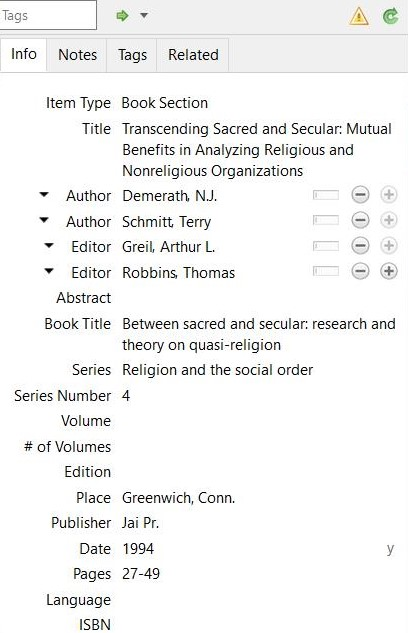
\includegraphics[keepaspectratio]{images/Zotero_Englisch.png}}
\caption{Entry in a literature database}
\end{figure}

The first step is to collect bibliographic data in the literature database. For this purpose, the information of a book, journal article or other text source is entered in general form. The later formatting does not play a role here. If the author is entered as “Weber, Max”, this can later be rendered “Weber, Max”, “Max Weber” or “Weber, M.”. The separation of meaning and formatting is similar to the formatting templates of a word processor, only the possibilities are much greater here.

It makes sense to link the collected references with the corresponding copy or file. In this way, it is easy to find a text that you read a long time ago. In principle, this is the structure of a small private library. Each copy must be provided with a short signature (e.g.~author and year of publication), which corresponds to the signature in the literature administration. If the copies are then filed according to signature, the matching text for an entry in the literature database can be found easily. In the case of electronic documents, this is usually even easier; here, the corresponding file can often be opened from the literature administration by pressing a button.

In connection with internet catalogs, some programs offer the possibility to import the literature data directly. This saves a lot of typing work, for example if an entry from a library catalog can be directly transferred to the literature administration.

\section{Output of Literature}\label{output-of-literature}

An important piece of work is taken off your hands if you leave the formatting of literature lists to the literature administration. This has several advantages:

\begin{itemize}
\item
  It is much faster,
\item
  the same literature list can easily be output in a completely different format,
\item
  one avoids careless mistakes and inconsistencies.
\end{itemize}

For this purpose, the programs usually provide a selection of ready-made formatting rules; if desired, you can create your own.

\begin{Tip}

If one uses such a program, it is usually sufficient to select a style that comes close to the specifications of the department. It is not necessary to create a style that exactly implements the guidelines.

\end{Tip}

\section{Embedding in Word Processing}\label{embedding-in-word-processing}

Most literature administration programs also offer the possibility to embed references directly into a document. In this way, not only the formatting of the bibliography can be controlled, but also the formatting of the references in the text. In addition, a list of the literature used in the text can be created automatically.

Usually Microsoft Word and often LibreOffice are supported by the commercial literature administration programs. LaTeX has its own literature management system, BibTeX, which is tightly integrated into LaTeX. The newer bibLaTeX also supports the more complicated conventions of the humanities.

\chapter{Visual Presentation}\label{sec:visual_presentation}

To support oral presentations, a visual presentation of key statements and/or illustrative materials is a good idea. Digital presentations have almost completely replaced overhead projectors or slide projectors. Although the term “PowerPoint presentation” shows the dominance of a particular product, it is misleading: screen presentations can be created using a variety of different tools.

The two large office packages, Microsoft Office and LibreOffice, contain programs for the design of on-screen presentations with \textbf{PowerPoint} and \textbf{Impress} respectively. These are very graphically oriented, so you can easily select different designs, insert graphics and dynamically display and animate individual elements. For the Office packages, see the note boxes in section \hyperref[sec:office]{Office Applications}.

\textbf{LaTeX} also contains components for creating on-screen presentations, such as LaTeX Beamer. Presentations created with LaTeX are more structure-oriented. This allows for automatic tables of contents or the highlighting of the current part of a presentation. For general information about LaTeX see the notes box in the section \hyperref[sec:latex]{LaTeX}.

In all cases, special attention must be paid to the fact that the technical possibilities of the software are intended to support the presentation, but are not an end in themselves. Thus, an on-screen presentation only makes sense for presentations of a certain length. An on-screen presentation is suitable for the following purposes:

\begin{itemize}
\item
  Writing down the core theses of the presentation in order to make it easier to follow the oral presentation,
\item
  graphic representation of complex facts that are difficult to convey in pure language (e.g.~diagrams, charts) and
\item
  support of the presentation with further media (e.g.~pictures, videos or audio documents).
\end{itemize}

Many presentation programs offer a wide range of options for designing slides and elements on slides. Especially fade-ins of text parts and fade-ins between slides can be animated in many ways. While these possibilities are exciting at first glance, on closer inspection their use is limited. A presentation gains from these effects when the attention of the audience is directed in a targeted manner. It loses when the attention is diverted from the content of the presentation. Too many visual gimmicks should therefore be avoided.

As effects may make sense:

\begin{itemize}
\item
  Inserts of enumerations to display key points only when they are mentioned in the presentation. This prevents the readers from reading in advance the contents that have not yet been mentioned in the presentation.
\item
  Step-by-step fade-in of diagrams.
\item
  Fade-ins between sections.
\end{itemize}

\begin{Technology}

On-screen presentations require a certain amount of technical effort during creation and presentation. It must be ensured that a projector and a computer are available on which the presentation can be played. For presentations of a few minutes the effort is therefore rarely justified. The choice of the appropriate file format is also important for presentations in order to avoid problems during playing:

\begin{itemize}
\item
  On most computers (but not on all) Microsoft PowerPoint is installed. However, different computers or different PowerPoint versions may cause shifts in the display.
\item
  LibreOffice Impress is not installed on all computers. Impress presentations can be saved in Microsoft PowerPoint format, but this may result in the loss of functions such as animations.
\item
  PDF files created from PowerPoint, Impress or LaTeX can be played almost everywhere. Only a PDF viewer such as Adobe Reader is required. In addition, a correct display in this format is guaranteed. However, animations and fade-in effects are lost when exporting to PDF.
\end{itemize}

In order to ensure the correct reproduction of on-screen presentations, it may therefore be advisable to bring your own laptop on which the presentation has been tested beforehand.

\end{Technology}

\begin{Remember}

\begin{enumerate}
\def\labelenumi{\arabic{enumi}.}
\tightlist
\item
  background, font and effects are kept simple and not overloaded
\item
  the font is sufficiently large.
\item
  at most one topic is treated per slide.
\item
  the slides are not overloaded with information.
\item
  In general, only the most important information is visualized, not every detail of the presentation.
\item
  In the oral presentation not only the points on the slides are read out.
\item
  Pictures, schemes, diagrams, charts, tables and statistics are to be discussed, not just for decoration.
\end{enumerate}

\end{Remember}

\end{document}
